\documentclass{astroedu-lab}

\begin{document}

\pagestyle{plain}

\begin{problem}{\huge Лабораторная работа 2.1.6\\\\Эффект Джоуля-Томсона\\\\Выполнил Жданов Елисей Б01-205}

\section{Цель работы:}

1) Определить изменения температуры углекислого газа при протекании через малопроницаемую перегородку при разных начальных значениях давления
и температуры. 

2) Вычислить по результатам опытов коэффициенты a и b модели Вандер-Ваальса.


\section{Оборудование:}

Трубка с пористой перегородкой

Труба Дьюара

Термостат жидкостной

Дифференциальная термопара

Вольтметр

Балластный баллон

Манометр

\section{Теоретическая справка}

Эффектом Джоуля–Томсона называется изменение температуры газа, медленно
просачивающегося из области высокого в область низкого давления.

Для газа можно записать уравнение Бернулли

\begin{equation}
	H_1 - H_2 = \frac{\mu}{2} \left( v_1^2 - v_2^2 \right)
\end{equation}

Пренебрегая кинетической энергией газа, получим

\begin{equation}
	H_1 \approx H_2
\end{equation}

Тогда имеет смысл обозначить коэффициент Джоуля-Томсона

\begin{equation}
	\mu = \frac{\Delta T}{\Delta P}
\end{equation}

Для газа Ван-дер-Ваальса можно записать приближенное выражение энтальпии

\begin{equation}
	H \approx C_p T + P \left( b - \frac{2 a}{R T} \right)
\end{equation}

Приравнивая её к нулю и рассматривая в рамках приращений, получим

\begin{equation}
	\boxed{\mu = - \frac{b - \frac{2 a}{R T}}{C_p}}
\end{equation}

Также обозначим температуру инверсии эффекта

\begin{equation}
	\boxed{T_\text{инв} = \frac{2 a }{R b}}
\end{equation}

%\subsection*{Экспериментальная установка}

\section{Установка}
Схема установки, используемой в работе приведена на рисунке\\
 
\begin{center}
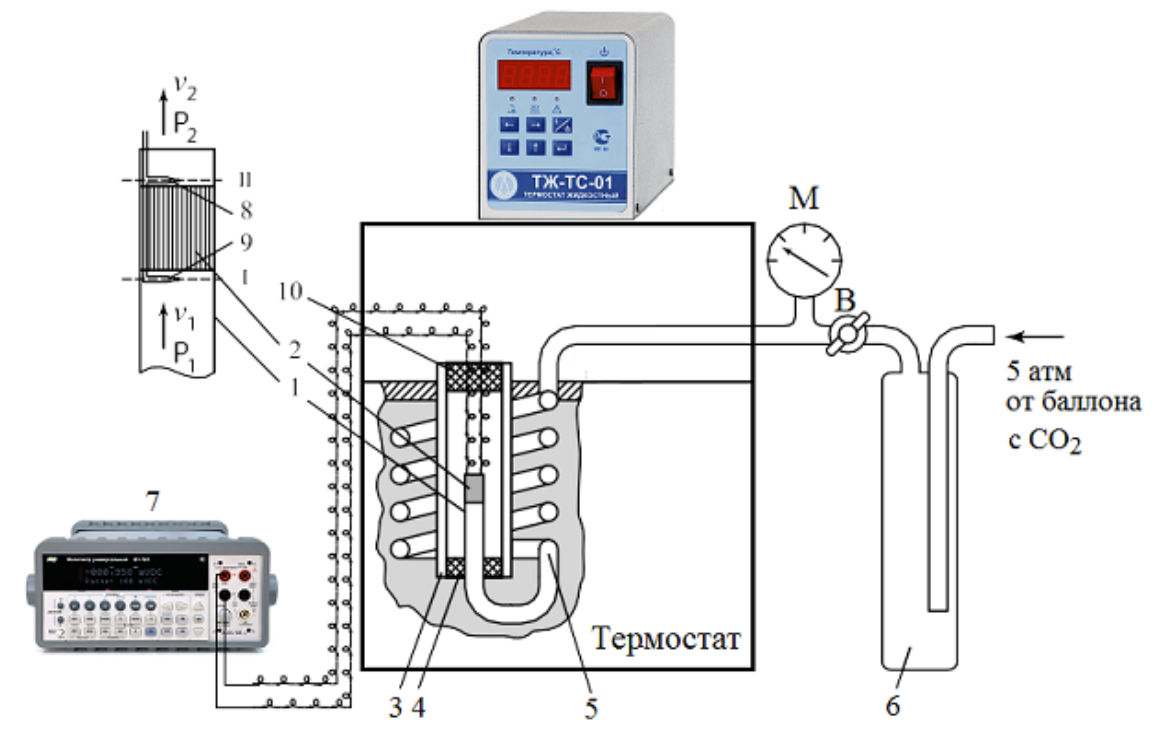
\includegraphics[width=0.8\textwidth]{st.png}
\label{ris:image}
\end{center}

Для замеров используется термометр на термостате, маниметр и термопара, подключенная к вольтметру.

\section{Измерения}

1-5) Запустим термостат и выставим на нем температуру, близкую к комнатной

Проверим, что вольтметр работает. Запишу его начальное показание

\begin{equation}
	U(0) = -0.007 \text{ мВ}
\end{equation}

6) Откроем кран, выставим давление в 4 бара.

7) Подождем 10 минут и запишем значение напряжения в таблицу

8-9) Проведем оставшиеся изменения и занесем значения в таблицу

\begin{center}
	$T = 22.08 ^\circ C$
\end{center}

\begin{center}
\begin{tabular}{|c|c|c|}
\hline
$\Delta P$, бар & $V$, мВ & $\Delta T$, C \\ \hline
4.0 & 0.0895 & $(2.39 \pm 0.07)$ \\
3.5 & 0.0715 & $(1.94 \pm 0.06)$ \\
3.0 & 0.0565 & $(1.57 \pm 0.06)$ \\
2.5 & 0.0420 & $(1.21 \pm 0.06)$ \\
\hline
\end{tabular}
\end{center}

\begin{center}
	$T = 30 ^\circ C$
\end{center}

\begin{center}
\begin{tabular}{|c|c|c|}
\hline
$\Delta P$, бар & $V$, мВ & $\Delta T$, C \\ \hline
4.0 & 0.0950 & $(2.48 \pm 0.07)$ \\
3.5 & 0.0780 & $(2.07 \pm 0.06)$ \\
3.0 & 0.0620 & $(1.68 \pm 0.06)$ \\
2.5 & 0.0475 & $(1.33 \pm 0.06)$ \\
\hline
\end{tabular}
\end{center}

\begin{center}
	$T = 40 ^\circ C$
\end{center}

\begin{center}
\begin{tabular}{|c|c|c|}
\hline
$\Delta P$, бар & $V$, мВ & $\Delta T$, C \\ \hline
4.0 & 0.0920 & $(2.36 \pm 0.07)$ \\
3.5 & 0.0775 & $(2.01 \pm 0.06)$ \\
3.0 & 0.0630 & $(1.67 \pm 0.06)$ \\
2.5 & 0.0510 & $(1.38 \pm 0.06)$ \\
\hline
\end{tabular}
\end{center}

\newpage

\begin{center}
	$T = 50 ^\circ C$
\end{center}

\begin{center}
\begin{tabular}{|c|c|c|}
\hline
$\Delta P$, бар & $V$, мВ & $\Delta T$, C \\ \hline
4.0 & 0.0900 & $(2.27 \pm 0.06)$ \\
3.5 & 0.0765 & $(1.95 \pm 0.06)$ \\
3.0 & 0.0635 & $(1.65 \pm 0.06)$ \\
2.5 & 0.0520 & $(1.38 \pm 0.06)$ \\
\hline
\end{tabular}
\end{center}

\begin{center}
	$T = 60 ^\circ C$
\end{center}

\begin{center}
\begin{tabular}{|c|c|c|}
\hline
$\Delta P$, бар & $V$, мВ & $\Delta T$, C \\ \hline
4.0 & 0.0855 & $(2.12 \pm 0.06)$ \\
3.5 & 0.0745 & $(1.87 \pm 0.06)$ \\
3.0 & 0.0635 & $(1.62 \pm 0.06)$ \\
2.5 & 0.0535 & $(1.39 \pm 0.06)$ \\
\hline
\end{tabular}
\end{center}

Систематическую погрешность манометра приму за 0.1 бар.

Пересчет $V$ в $\Delta T$ произведем с помощью линеарицации соответствующего графика для термопары

\begin{center}
\begin{tabular}{|c|c|}
\hline
$T$, С & $E$, мкВ/С \\ \hline
22 & 40.44 \\
30 & 41.10 \\
40 & 41.95 \\
50 & 42.80 \\
60 & 43.65 \\
\hline
\end{tabular}
\end{center}

Погрешность составляет $0.3$ мкВ$/ ^\circ$C

\begin{center}
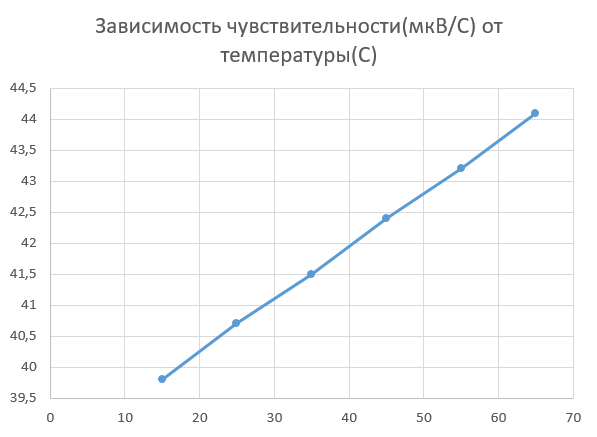
\includegraphics[width=0.8\textwidth]{термо.png}
\label{ris:image}
\end{center}

\section{Обработка}

10) Построим на одном графике зависимости $\Delta T$ от $\Delta P$

\begin{center}
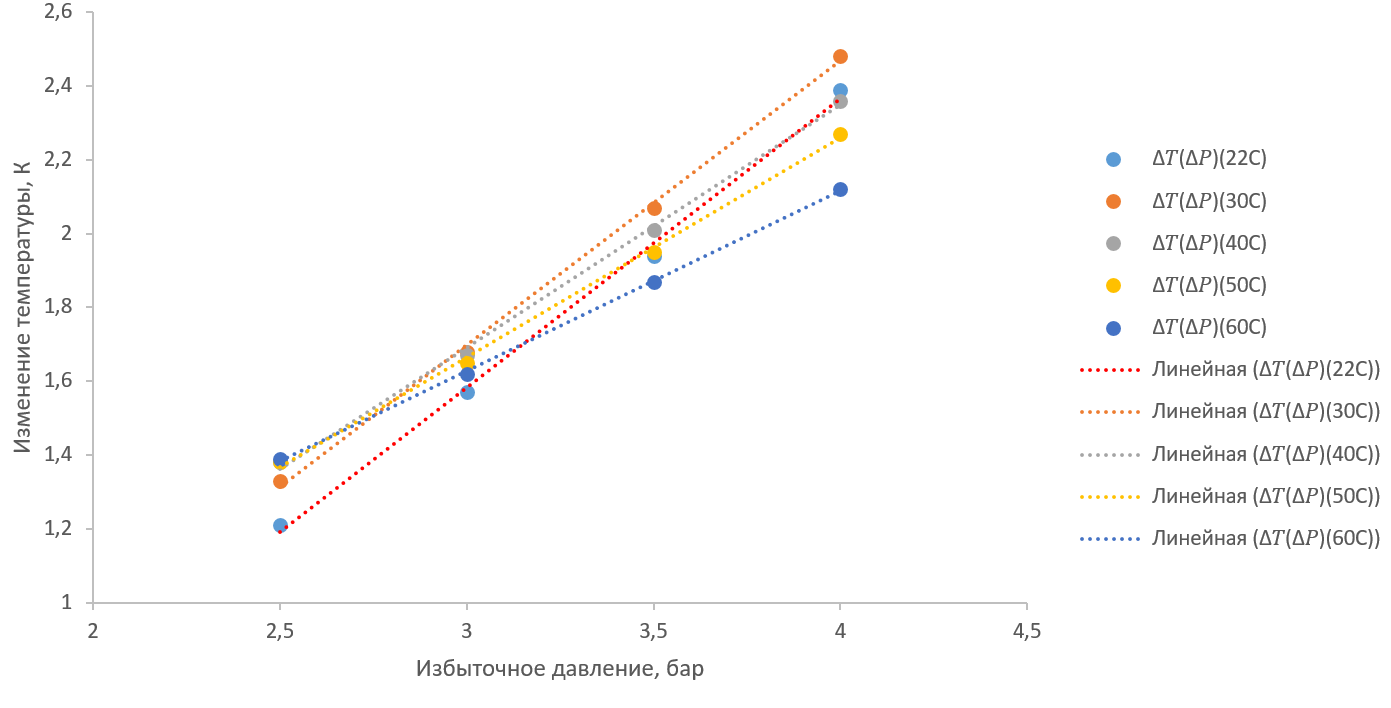
\includegraphics[width=1\textwidth]{1_plot.png}
\label{ris:image}
\end{center}

Полученные коэффициенты Джоуля-Томсона занесем в таблицу

\begin{center}
\begin{tabular}{|c|c|}
\hline
$\mu$, $\frac{\text{К}}{\text{бар}}$ & T, K \\ \hline
$(0.782 \pm 0.030)$ & 22 \\
$(0.768 \pm 0.019)$ & 30 \\
$(0.656 \pm 0.020)$ & 40 \\
$(0.594 \pm 0.016)$ & 50 \\
$(0.488 \pm 0.007)$ & 60 \\
\hline
\end{tabular}
\end{center}

11) Построим итоговый график

\begin{center}
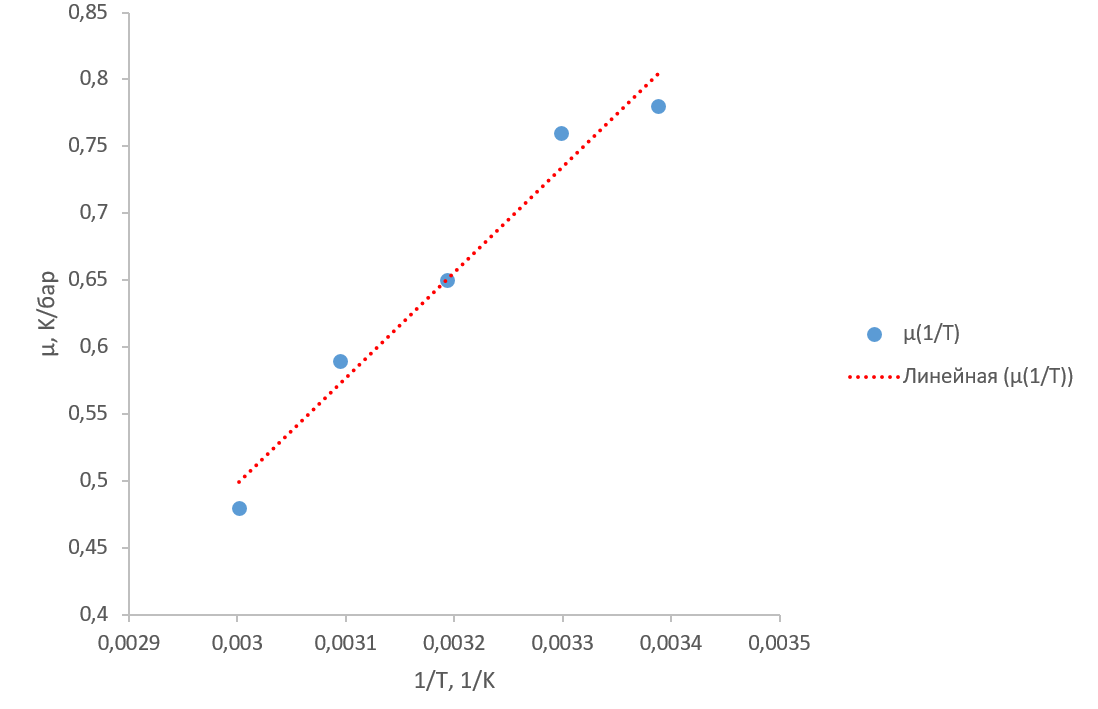
\includegraphics[width=1\textwidth]{main_plot.png}
\label{ris:image}
\end{center}

Формулы используемого МНК

\[
	a = \frac{<x_i y_i> - < x > < y_i >}{< x_i^2> - < x_i >^2}
\]

\[
	b = < \nu_i > - a < N_i >
\]

Погрешности величин

\begin{equation}
	S_a^2 = \frac{< x_i^2>}{< x_i^2 > - < x_i >^2} \cdot \frac{<  b_i - b > ^2}{n - 2}
\end{equation}

В итоге уравнение прямой 

\begin{equation}
	\mu = (-1.87 \pm 0.26) + \frac{(789 \pm 83)}{T} = p + \frac{q}{T}
\end{equation}

Принимая значение теплоемкости углекислого газа $C_p = 37.1 \frac{\text{Дж}}{\text{моль $\cdot$ K}}$, получим коэффициенты

\begin{equation}
	a = \frac{q C_p R}{2} = (1.20 \pm 0.13) \frac{\text{H $\cdot$ м}^4}{\text{моль}^2}
\end{equation}

\begin{equation}
	b = - p C_p = (680 \pm 90) \frac{\text{см}^3}{\text{моль}}
\end{equation}

Теоритечские же значения

\begin{equation}
	a = \frac{q C_p R}{2} = 0.36 \frac{\text{H $\cdot$ м}^4}{\text{моль}^2}
\end{equation}

\begin{equation}
	b = - p C_p = 43 \frac{\text{см}^3}{\text{моль}}
\end{equation}

Рассчитаем температуру инверсии

\begin{equation}
	T_\text{инв} = \frac{2 a}{R b} = (430 \pm 120) \text{ K}
\end{equation}

Табличное

\begin{equation}
	T_\text{инв} = 2000 \text{ K}
\end{equation}

\section{Вывод}

Полученные экспериментальные данные в разы отличаются от табличных данных. Это говорит ни о чем ином, как о расхождении эксперимента с теорией. То есть полученные коэффициенты могут разумно описывать поведение газа при дросселировании, но при этом давать совершенно некорректные показания в других экспериментах. Улучшить соответствие можно использованием более точной теоретической модели, либо в какой-то степени совершенствованием экспериментальной установки.

\end{problem}
\end{document}